\documentclass[a4paper, 11pt]{report}
\usepackage{blindtext}
\usepackage[T1]{fontenc}
\usepackage[utf8]{inputenc}
\usepackage{titlesec}
\usepackage{fancyhdr}
\usepackage{geometry}
\usepackage{fix-cm}
\usepackage[hidelinks]{hyperref}
\usepackage{graphicx}
\usepackage{titlesec}
\usepackage{hyperref}
\usepackage{url}


\usepackage[english]{babel}

\geometry{ margin=30mm }
\counterwithin{subsection}{section}
\renewcommand\thesection{\arabic{section}.}
\renewcommand\thesubsection{\thesection\arabic{subsection}.}
\usepackage{tocloft}
\renewcommand{\cftchapleader}{\cftdotfill{\cftdotsep}}
\renewcommand{\cftsecleader}{\cftdotfill{\cftdotsep}}
\setlength{\cftsecindent}{2.2em}
\setlength{\cftsubsecindent}{4.2em}
\setlength{\cftsecnumwidth}{2em}
\setlength{\cftsubsecnumwidth}{2.5em}

\titlespacing\section{0pt}{12pt plus 4pt minus 2pt}{0pt plus 2pt minus 2pt}
\titlespacing\subsection{0pt}{12pt plus 4pt minus 2pt}{0pt plus 2pt minus 2pt}
\begin{document}
\titleformat{\section}
{\normalfont\fontsize{15}{0}\bfseries}{\thesection}{1em}{}
\titlespacing{\section}{0cm}{0.5cm}{0.15cm}
\titleformat{\subsection}
{\normalfont\fontsize{13}{0}\bfseries}{\thesubsection}{0.5em}{}
\titlespacing{\section}{0cm}{0.5cm}{0.15cm}

%=============================================================================

\pagenumbering{Alph}
\begin{titlepage}
\begin{flushright}

\includegraphics[width=4cm]{USyd}\\[2cm]
\end{flushright}
\center 
\textbf{\huge INFO1111: Computing 1A Professionalism}\\[0.75cm]
\textbf{\huge 2023 Semester 1}\\[2cm]
\textbf{\huge Self-Learning Report}\\[3cm]

\textbf{\huge Submission number: 1}\\[0.75cm]
 \textbf{Github link: https://github.com/Iambehindyou2/Info1111-Self-Learning}\\[2cm]

{\large
\begin{tabular}{|p{0.35\textwidth}|p{0.55\textwidth}|}
	\hline
	{\bf Student name} & Kailin Zhang\\
	{\bf Student ID} & 5305576006\\
	{\bf Topic} & PHP \\
	{\bf Levels already achieved} & X\\
	{\bf Levels in this report} & A\\
	\hline
\end{tabular}
}
\thispagestyle{empty}
\end{titlepage}
\pagenumbering{arabic}
%=============================================================================
\newpage
\section{Level A: Initial Understanding}
\vspace{5mm}
\subsection{Level A Demonstration}
\begin{itemize}
  \item The Installation of PHP and the IDE/Code editor in order to write in PHP. This includes getting familiar with PHP basic syntax and able to write simple PHP script
  \item Using PHP to connect to simple databases, this may include filtering, displaying and counting data etc
  \item Learning Object-oriented programming of PHP
\end{itemize}

\subsection{Learning Approach}

In the very beginning, before I selected my self-learning topic, I conducted some simple research on all the options available. I discovered that I had an interest in cybersecurity and PHP was a popular language for web development and back-end, so I chose it as my topic. Although I had zero knowledge of PHP, I first watched some brief introduction videos on YouTube to gain some basic knowledge. After understanding what PHP is, I searched for a tutorial on installation. Personally, I believe that learning without practical application is worthless because people will soon forget what they've learned. I like to learn by practising on my own to gain a better understanding. After I installed PHP and the IDE and was ready to go, I found a website called "w3school" that provided detailed knowledge and lectures on PHP. I went through the lectures while referring to a five-hour video on YouTube that talked about PHP. I found that incorporating videos and lectures helped me learn better.

\subsection{Challenges and Difficulties}

I think in general all computer languages, no matter which ones, are a challenge for me because I don’t have experience with using them. After selecting the PHP, I found out that the PHP coding language is like a big ZIP file, it also contains HTML, MYSQL and other languages or forms of coding. For instance, using the level A self-learning as an example, in order for me to create an actual web I have to use HTML. However, at the same time I have to embed the PHP into the file in order for users to input value and also for “me” to receive the value. Connecting the database is like on a different level to be honest, personally speaking I think that is for level B and above. Because it requires knowledge toward using MYSQL and that is like another different set of coding. I already downloaded “DataGrip” and am exploring how to use DataGrip to manipulate SQL files and connect through with PHP.

\subsection{Learning Sources}
\begin{itemize}
  \item \url{https://www.youtube.com/watch?v=OK_JCtrrv-c&t=2640s}{This is a 5 hour video explaining and tutoring on PHP, it helped me a lot with all the syntax and functions of PHP}\cite{PHP}
  \item \url{https://www.youtube.com/watch?v=a7_WFUlFS94}{This is a short video briefly introducing PHP overall}\cite{PHP100}
  \item \url{https://www.bilibili.com/video/BV18x411H7qD/?spm_id_from=333.337.search-card.all.click}{This is also a very detailed tutoring video on PHP, it helped me a lot on making the local host as the server}\cite{HM}
  \item \url{https://www.w3schools.com/php/php_math.asp}{This is a lecture in text, going through all types of math, functions, data type and all other syntax}\cite{W3}
\end{itemize}



%=============================================================================

\newpage
\subsection{Application artifacts}

Installation of PHP and IDE:
I first installed Homebrew on my MAC OS by running the command “/bin/bash -c and then installed PHP by running the command “brew install php”. After adding the Homebrew PHP path to my path, I was able to use PHP.

Creating a local server:
To create a local server, I navigated to the directory where I had saved my PHP file and ran the command “Php -S localhost:4000”. This created a local server that I could use to make a simple webpage by copying the URL to my Chrome.

Creating a login page and calculator:
After successfully creating a local server and linking to the PHP file, I created a simple login page that allowed users to input their username and password. I used signing values to variables, if function and method post to hide the URL parameter. If the password and username were not valid, it would display invalid information. Additionally, I also coded a simple calculator that could perform operations such as addition, subtraction, multiplication, and division. The user could input different numbers and then click on the operation they wanted to perform.

Commenting in the coding document:
To further explain my work, I used // for PHP and <! …….--> for HTML to add comments to the coding document.

Challenges faced:
One of the problems I faced was that the calculator and login page could not operate separately. This meant that both would output at the same time, and I currently do not know how to fix it. However, I am still learning and making progress on PHP.

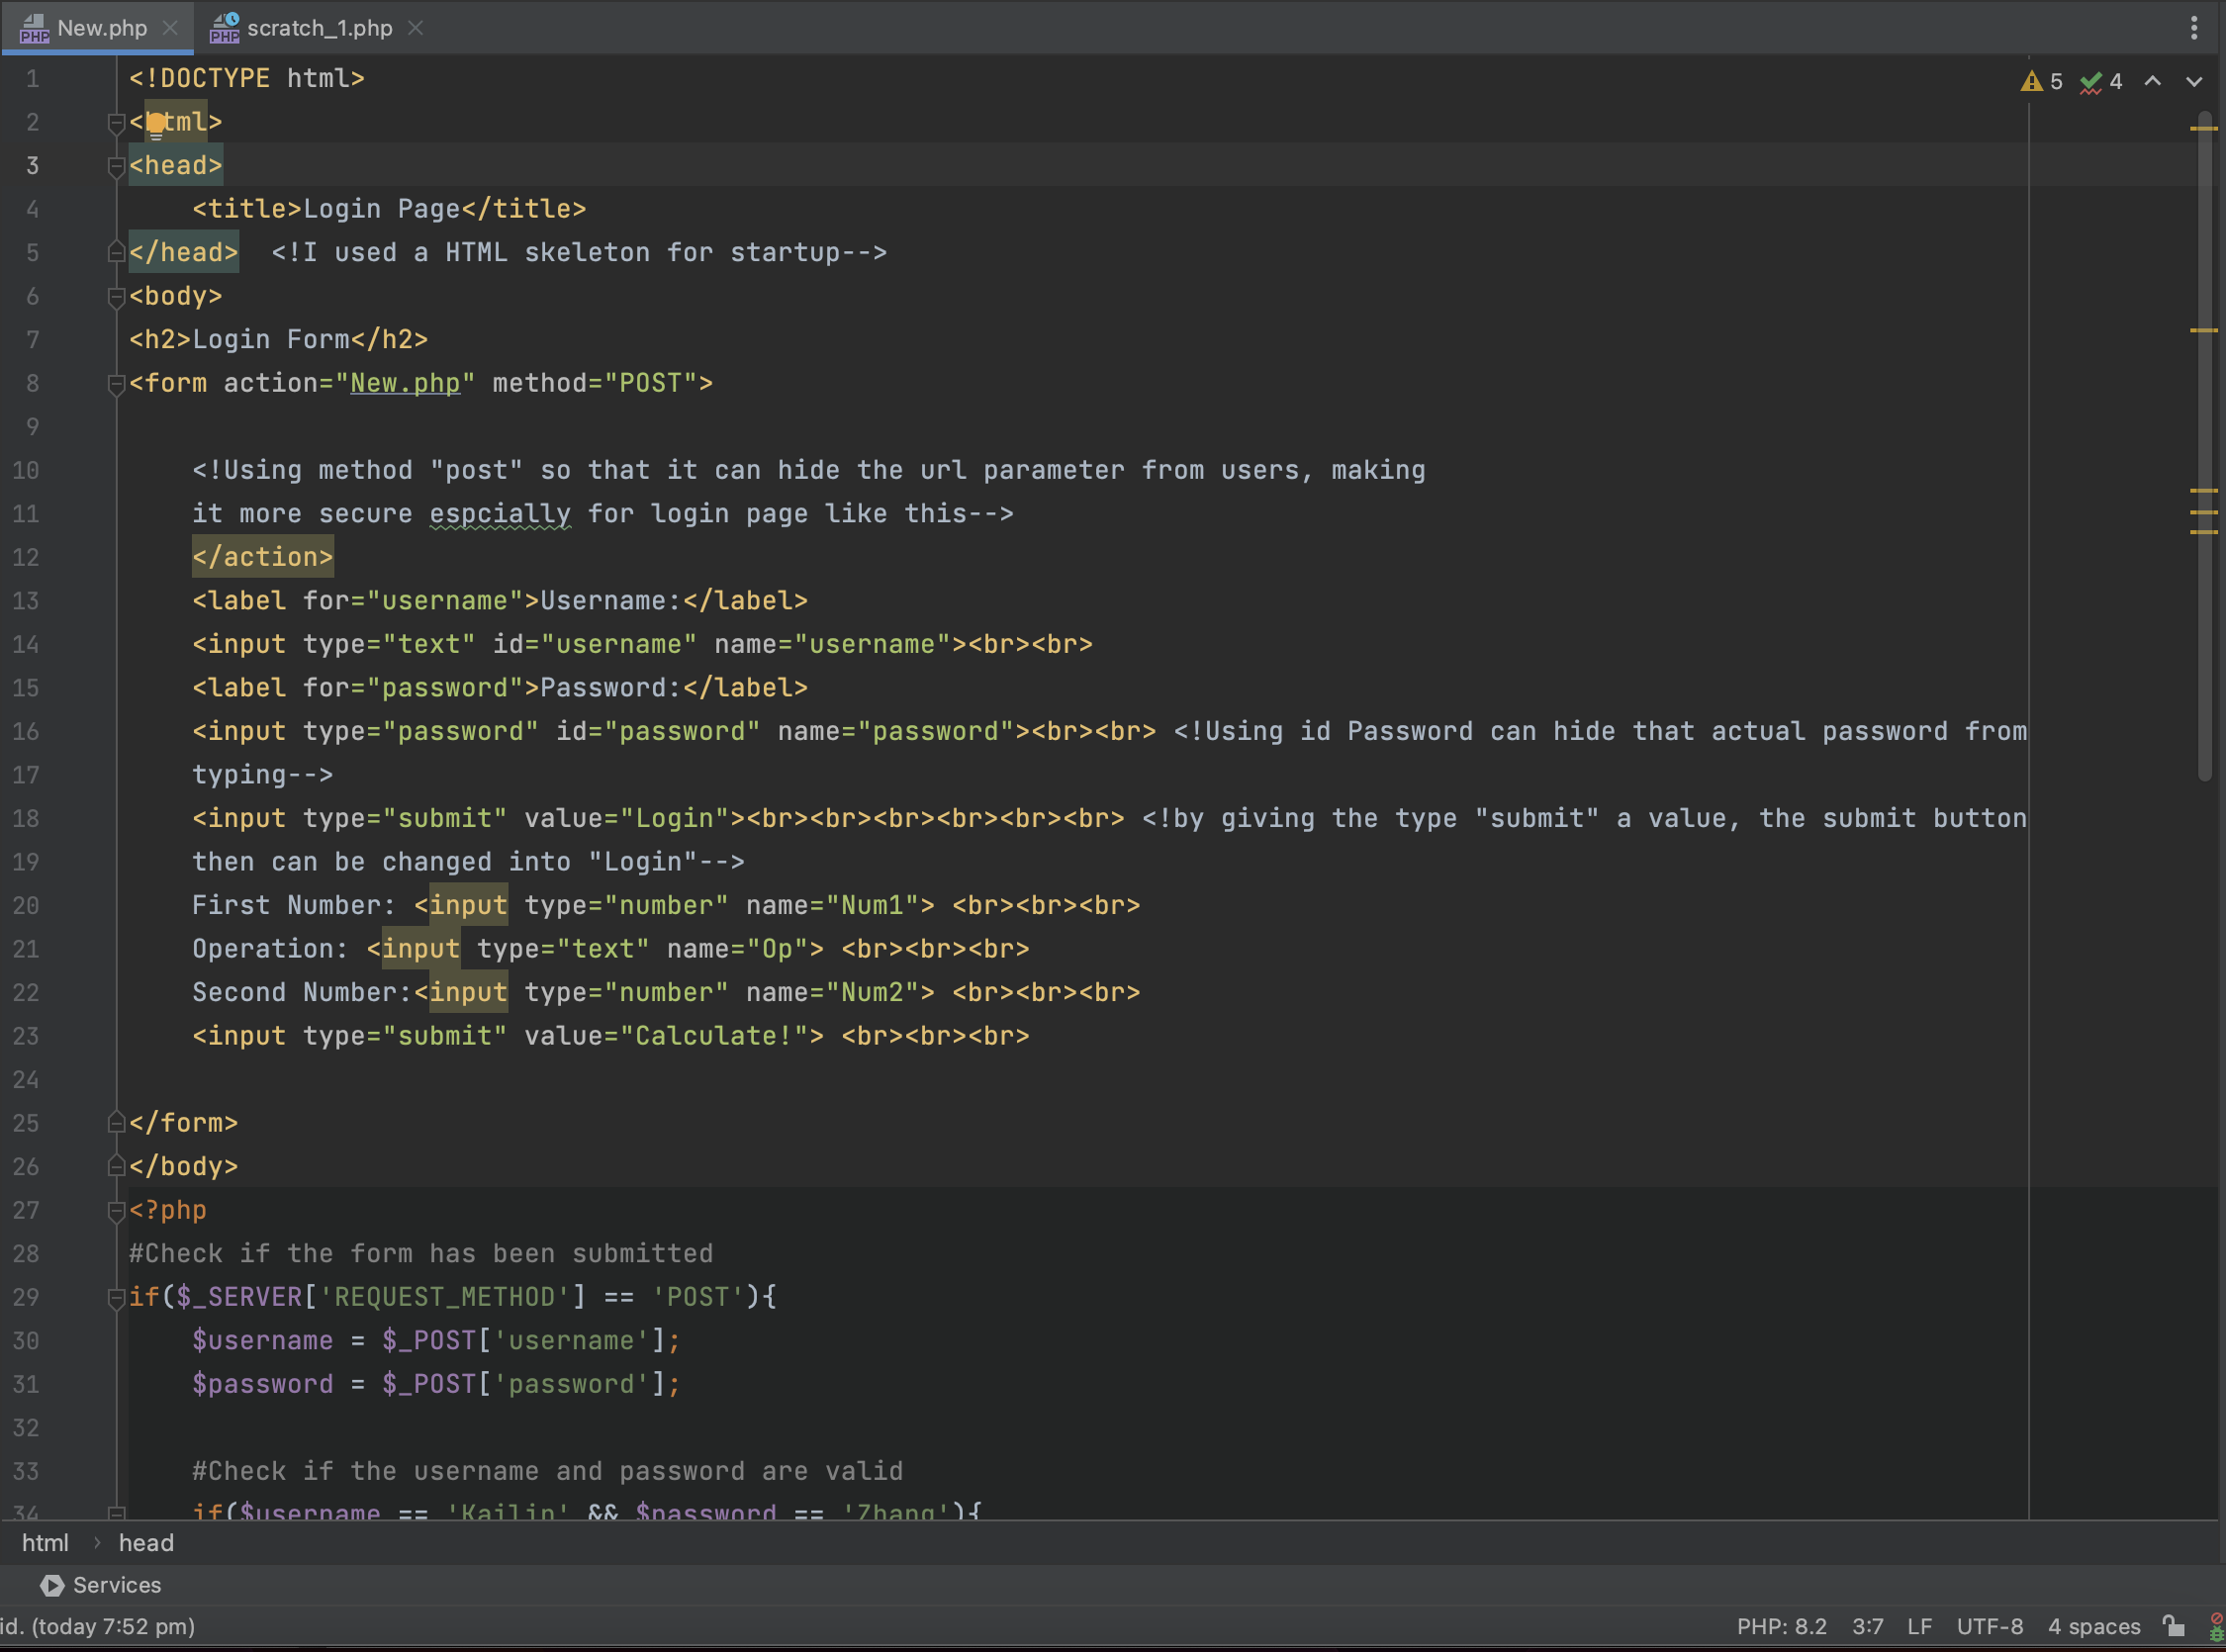
\includegraphics[width=1\textwidth]{1}
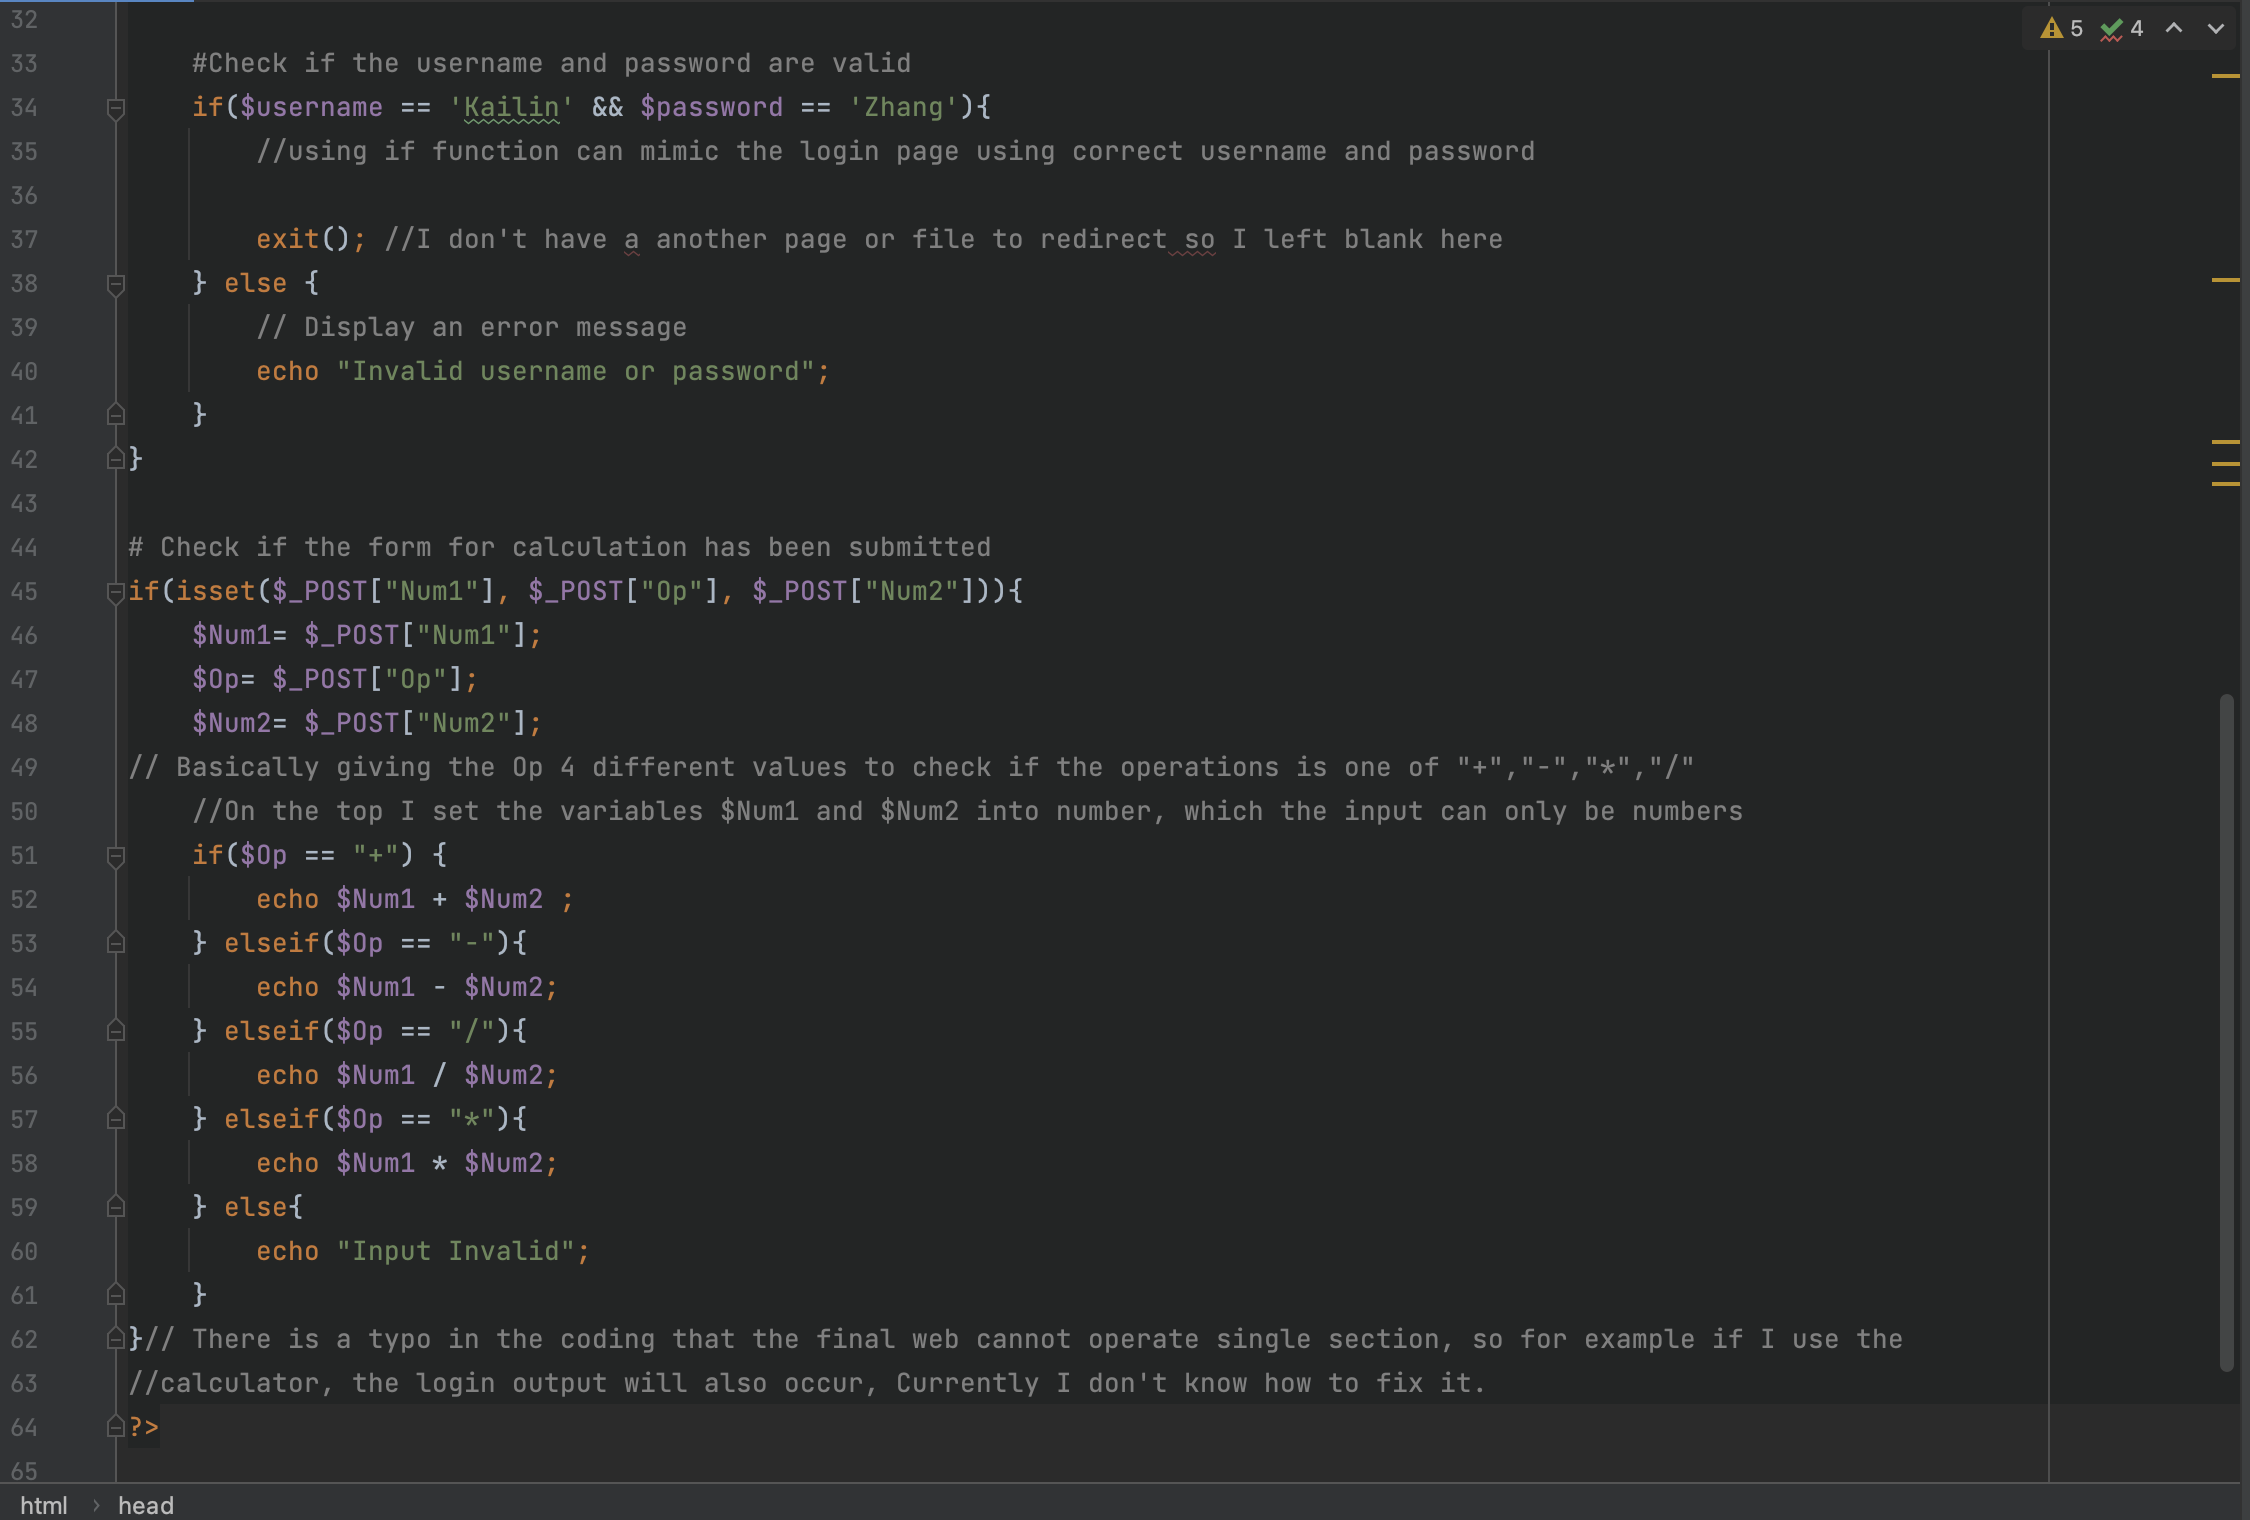
\includegraphics[width=1\textwidth]{2}

%=============================================================================
\newpage
\bibliographystyle{IEEEtran}
\bibliography{123}


\end{document}


\end{document}
\end{report}
